\section*{Lecture \# 6: Lyapunov Stability of Equilbium}


Given the system...


$$
\dot{x} = f(x) \quad \quad \text{ and input } u = k\cdot x
$$

\noindent Such that...

$$
\dot{x} = f(x,u) = f(x, k(x)) :=f(x)
$$

\noindent Where the function is defined from

$$
f: D \rightarrow \R^n
$$

\noindent Where $D\subset \R^n$. Addition, the system is understood to be \textbf{locally Lipschitz Continuous}, such that.

$$
\left\Vert f(x) - f(y) \right\Vert \leq L \left \Vert x - y \right\Vert
$$

\noindent Without loss of generality, we can write that $ \bar{x} = 0
$, is an \underline{equilibrium point} of the system $\bar{f}(x)$ such that when evaluated at the point $\bar{x} = 0$, then $\bar{f}(\bar{x}) = f(0) = 0 $

\subsection*{Conditions for Stability}

We can call the given system \underline{stable} if..

$$
\forall \epsilon > 0 \text{ , } \exists \delta = \delta(\epsilon) > 0
$$

\noindent Such that...

$$
\left\Vert x(0)\right\Vert < \delta \quad \Rightarrow \quad \left\Vert x(t)\right\Vert < \epsilon \text{ , } \forall t \geq 0
$$

\subsubsection*{\underline{Stability Explaination}}

In order for the system to be \underline{stable} we must be able to demonstrate in a rigorous $\epsilon-\delta$ fashion that, there exists some domain in which, if a trajectory is begun inside of ball $\delta$, the trajectory will be maintained inside of ball $\epsilon$, for all positive time greater than the initial condition.


\subsection*{Conditions for Instability}

Conversely, the system is \underline{unstable} if...

$$
\forall \epsilon > 0 \text{ , } \exists \delta = \delta(\epsilon) > 0
$$

\noindent Such that...

$$
\left\Vert x(0)\right\Vert < \delta \quad \Rightarrow \quad \left\Vert x(t)\right\Vert \geq \epsilon \text{ , } \forall t \geq 0
$$


\subsubsection*{\underline{Instability Explaination}}

Unlike the case for stability, we can show using the same mathematical formulation that a system is \underline{unstable} if inside a ball of radius $\delta$, the trajectory cannot be maintained inside of a finite ball of radius $\epsilon$, for all time.


\subsection*{Examples of Stability vs Instability}

\subsubsection*{Stable Trajectory}
As shown using the $\epsilon-\delta$ balls, any trajectory which starts with initial conditions inside the ball $\delta$, there exists an $\epsilon$ such that the solution is bounded by $\epsilon$. This is an example of \underline{stable} behavior.


\begin{center}
  \includegraphics[scale=0.5]{lecture6_img/stable}
\end{center}

\subsubsection*{Saddle Point}

A saddle point is clearly unstable visually, when inspecting the phase portrait of the system, since there exist trajectories which diverge asymptotically to $\pm \infty$. Even though the origin, demonstrates stable behavior there does not exist a $\epsilon-\delta$ neighborhood, such that the trajectories in that neighborhood converge to the origin, or stay inside of the defined bounds. \\

\begin{center}
  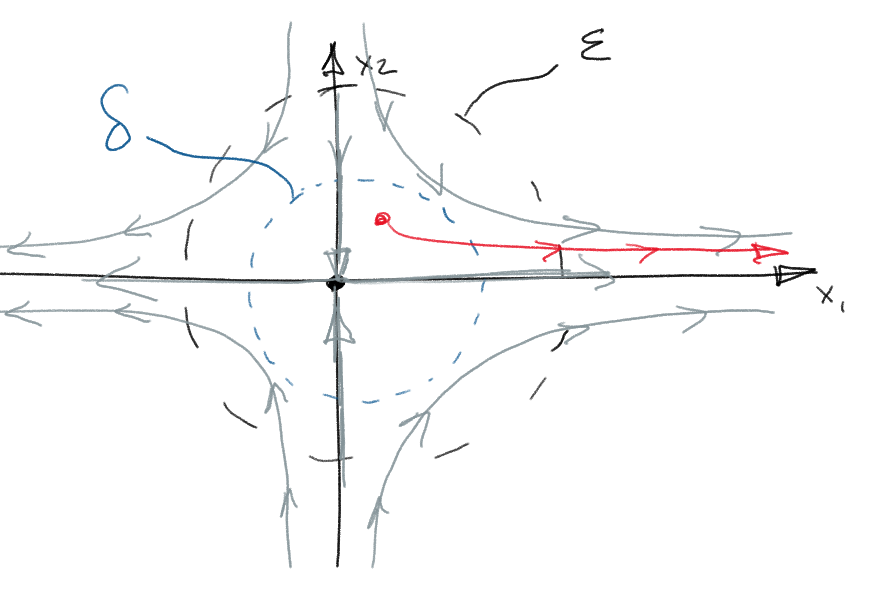
\includegraphics[scale=0.35]{lecture6_img/saddle}
\end{center}

\subsubsection*{Homoclinic Orbit}
While the previous examples are fairly obvious, there are a great many number of nonlinear system which exhibit strange behavior, and require further description. \\

\noindent For example, the concepts of \underline{domain of attraction} and \underline{asymptotic stability}, do not always go hand in hand.

\begin{itemize}
  \item \textbf{\underline{Attractive:}}  \\ A system is attractive if... \\ $\quad \exists \:\: \bar{\delta} >0 \text{ s.t. } \left \Vert x(0) \right\Vert <\bar{\delta} \Rightarrow x(t) \rightarrow 0 \text{ as } t \rightarrow 0$

  \item \textbf{\underline{Asymptotically Stable:}} Stable \& Attractive \\
\end{itemize}


\begin{center}
  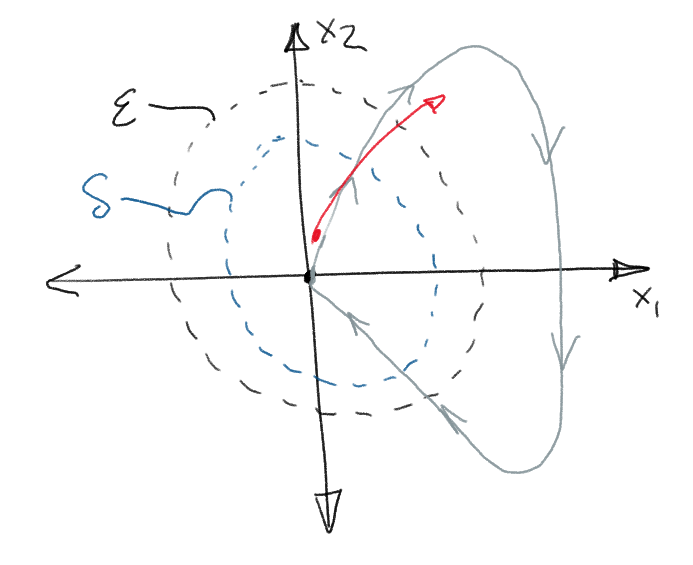
\includegraphics[scale=0.40]{lecture6_img/homoclinic}
\end{center}

\noindent The image above, is the phase portrait of a  \underline{homoclinic orbit} that is attractive but \textbf{NOT} stable. For this system, even though the system is \underline{attractive}, it is impossible to define a $\epsilon-\delta$ neighborhood which is stable since the trajectories shoot out before coming back to the origin. Therefore, even though the system is not stable it is simultaneously  not attractive.

\subsection*{Global Stability}
There also exist systems which are \underline{globally stable}. This property is defined as follows.

\noindent A system is \underline{globally stable} if, in addition to being \underline{stable} over the domain $D \subset \R^n$ it follows that ...

$$
\text{Given } \delta>0 \text{,  }\: \exists \: \epsilon = \epsilon(\delta) > 0$$

$$ \text{ s.t.} \left\Vert x(0) \right\Vert < \delta \Rightarrow \left\Vert x(t) \right\Vert < \epsilon \quad \forall t \geq 0
$$

$$
\text{Such that } B_r = \{ x \in \R^n : \left\Vert x \right\Vert \leq \delta \}
$$

\subsubsection*{Global Stability Explaination}
While local stability required the $\epsilon-\delta$ neighborhood to exist for some domain $D$ which is a subset of the real-numbers, \underline{global stability}, dictates that there must exist an $\epsilon-\delta$ neighborhood for the entire domain of the state space.

\subsection*{Types of Global Stability}


\begin{itemize}
  \item \textbf{\underline{Globally Stable}} \\

  A system is globally stable if it satisfies the definition given above, such that any for any initial state in the domain $\R^n$ the trajectories of the system are bounded.

  \item \textbf{\underline{Globally Attractive}} \\

  A system is globally attractive if $x(t) \rightarrow 0 \text{ as } t \rightarrow \infty$ for all $x(0) \in \R^n$. (If the system is attractive throughout the entire state space)

  \item \textbf{\underline{Globally Asymptotically Stable}} \\

  A system is globally asymptotically stable if it is ... \\

  \begin{enumerate}
    \item Globally Attractive
    \item Globally Stable
  \end{enumerate}

  \item \textbf{\underline{Exponentially Stable}} \\

  A system, is exponentially stable if ...

  $$
\exists \; C \text{, } K \text{, } \lambda > 0 \text{ s.t. }
  $$

  $$
  \left\Vert x(t) \right\Vert \leq K \left\Vert x_0 \right\Vert e^{\left( -\lambda\cdot t \right)}
  $$
\end{itemize}


\subsection*{Assessing Stability}

Given the system...

$$
\dot{x} = f(x)
$$

\noindent About the equilibrium point $x_0 = 0$ such that..

$$
\dot{x} = f(x_0) = 0
$$

\noindent We can establish \underline{local stability} on the basis of linearization of the system, about the equilibrium point such that...

$$
 \dot{y} = A y \quad \quad \text{where } y:= x -x_0
$$

\noindent Where the matrix $A$, is the jacobian of the system and is defined as ...
$$
 A =
  \begin{bmatrix}
    \frac{\partial f_1}{\partial x_1} & \cdots \frac{\partial f_1}{\partial x_n} \\
    \frac{\partial f_n}{\partial x_1} & \cdots \frac{\partial f_n}{\partial x_n} \\
   \end{bmatrix}
$$

\subsection*{Lyapunov's Indirect Method}
This linear approach to finding the stability of a nonlinear system is known as \underline{Lyapunov's Indirect Method}. In effect, this method is making local generalization about the stability of the nonlinear system due to its linear characteristics. \\

\noindent Since linear systems can be characterized via eigenvalues, we can use standard definitions of stability using classical control theory as follows...

\begin{enumerate}
  \item \textbf{\underline{Local Asymptotic Stability: }} \\

  We can conclude a linearized system is L.A.S. if...

  $$
  \text{Re}(\lambda_i) < 0 \quad \quad \forall i \in \left[ i, \cdots n  \right]
  $$

  \item \textbf{\underline{Unstable: }} \\

  We can condlude a linearize system is unstable if at least one $\text{Re}(\lambda_i) > 0$, at the equilibrium point $x = 0$.

  \item \textbf{\underline{No Determination: }} \\

  We \underline{cannot determine} the stability of the system if lat least one $\text{Re}(\lambda_i) = 0 $
\end{enumerate}



\subsection*{Alternative Approach for Assessing Stability}

The motivating example for this alternative approach is to understand the physical implications of the system. To understand this, we will look at a \underline{Pendulum with Friction}, where the states of the system are $x_1 = \theta $ and $x_2 = \dot{\theta}$.

$$
\begin{array}{l}
\dot{x}_{1}=x_{2} \\
\dot{x}_{2}= -\left( \frac{g}{l} \right) \cdot Sin(x_1) - \frac{k}{m}x_2
\end{array}
$$

\noindent We know that energy of physical systems must be conserved. Therefore, we know that give that our system has \underline{friction}, a form of energy dissipation, that the system must inherently trend towards $0$. We can use this intuition from the physical system and compute the energy of the system which takes the form of a scalar equation from which will act as the stand-in for a larger more well defined class of functions that will facilitate more rigorous analysis.

$$\text{Energy = PE + KE}$$
$$
\quad = \int_{0}^{x_1} \left( \frac{g}{l} \right) \cdot Sin(x_1) ds + \frac{1}{2} x_2^2
$$

$$
\quad = \frac{g}{l} \left[ 1 - Cos(x_1) \right] + \frac{1}{2} x_2^2
$$


\noindent This type of analysis will provide a valuable perspective later when analyzing the stability of more complicated and non-trivial systems.
